\documentclass[a4paper,11pt]{article}

\usepackage[utf8]{inputenc}

\usepackage{graphicx}
\usepackage{caption}
\usepackage{subcaption}

\usepackage{pgfplots}
\pgfplotsset{compat=1.18} 

\usepackage{minted}
\usepackage{siunitx}

\begin{document}

\title{
    \textbf{Linked lists in C}
}
\author{Mo Wang}
\date{Spring 2026}

\maketitle

\section*{Introduction}
This report investigates and delves into performance and behavior of a linked list in C. While linked list offers flexibility by carrying an address of next element of a list, it has some performance bottlenecks in terms of random access and cache locality. The primary goal of this report is to analyze the behavior and key attribute of a linked list and compare these features with arrays.


\section*{Linked list}

A linked list stores a sequence of elements by holding its first element. Each element in a linked list is stored in a cell with an element value and a pointer with the address of the next cell. A null pointer in a linked list cell denotes the last cell in the list, while a null pointer as the first element denotes the absence of elements in the list.

\begin{minted}{c}
typedef struct cell {
    int value;
    struct cell *tail;
} cell;

typedef struct linked {
    cell *first;
} linked;
\end{minted}

The linked list can be created by allocating a memory for the linked list and successively allocating other cells of the list, where one cell address is stored in the previous one's tail. 

A linked list is created by first allocating memory for the list structure itself. Each cell is then successively allocated with each cell's tail pointer storing the address of the next cell in the sequence, hence linking all the cells together. The linked list structure stores a pointer to the first cell as an entry point to the data structure- From a memory perspective, these cells are scattered in dynamic memory, which provides flexibility at the expense of high performance overhead of accessing and searching operations.

\begin{minted}{c}
linked *linked_create() {
    linked *new = (linked*)malloc(sizeof(linked));
    new->first = NULL;
    return new;
}
void linked_free(linked *lnk) {
    cell *nxt = lnk->first;
    while (nxt != NULL) {
        cell *tmp = nxt->tail;
        free(nxt);
        nxt = tmp;
    }
    free(lnk);
}
\end{minted}

\subsection*{Adding an element}

To insert an element at the beginning of a linked list, a new cell is first allocated. The value of the new cell is assigned to the desired element. Its tail pointer is then assigned to point to the current first cell of the list. Finally, the first pointer of the list is updated to point to this new cell, effectively making it the first element of the list. Since the operation requires only one memory allocation and three pointer updates, the time complexity is constant $O(1)$.

\begin{minted}{c}
void linked_add(linked *lnk, int item) {
    cell *new = (cell*) malloc(sizeof(cell));
    new->value = item;
    new->tail = lnk->first;
    lnk->first = new;
}
\end{minted}

\subsection*{Length of linked list}

Because this implemented linked list structure only stores a pointer to first element cell without other necessary metadata, such as the size of the list, calculating the length of the linked list could only be accomplished by traversing the linked list through all the cells. A length counter is held and increments when moving to another cell through the previous cell's tail pointer during traversal. As all cells must be traversed, the complexity of the operation in time is linear to the size of the list $O(n)$.

\begin{minted}{c}
unsigned int linked_length(linked *lnk){
    unsigned int length = 0;
    cell* nxt = lnk->first;
    while (nxt != NULL){
        nxt = nxt->tail;
        length++;
    }
    return length;
}
\end{minted}

\subsection*{Finding an element}

Finding an element requires traversing the linked list from the first element cell to the last one, since the list can only be efficiently accessed sequentially. In this case, the value of each element cell is compared with the search value. The traversal search stops as the element is found. This results in linear time complexity $O(n)$, since each cell has to be traversed in the worst case, while only one cell is traversed in the best case. The operation performs on average $n/2$ traversal in terms of possibility expectation.

\begin{minted}{c}
bool linked_find(linked *lnk, int item){
    cell *nxt = lnk->first;
    while (nxt != NULL && nxt->value != item){
        nxt = nxt->tail;
    }
    return nxt != NULL;
}
\end{minted}

\subsection*{Removing an element}

An element can be removed by finding the element cell by value and therefore unlink it from adjacent cells. The operation is split into two cases: either the first element is targeted for deletion, or the deleted element is in the middle of the list. Removing the first element can be accomplished by updating the first pointer of linked list to the second cell while freeing the first cell. Meanwhile, removing an element in the middle of the array requires finding the element by tracking its previous cell. As the target element cell is found, the previous cell re-links its tail to the element after the target one, while freeing the target afterwards. Although pointer updates and free operations are done in constant time, the target element cell must be located by finding, resulting in linear time complexity $O(n)$, as described earlier.

\begin{minted}{c}
void linked_remove(linked *lnk, int item){
    cell *nxt = lnk->first;
    if (nxt == NULL) return;
    if (nxt->value == item){
        cell *after = nxt->tail;
        free(nxt);
        lnk->first = after;
    }
    else{
        while (nxt->tail != NULL && nxt->tail->value != item){
            nxt = nxt->tail;
        }
        if (nxt->tail != NULL){
            cell *after = nxt->tail->tail;
            free(nxt->tail);
            nxt->tail = after;
        }
    }
}
\end{minted}

\section*{Benchmark of append operation}
\subsection*{Append Implementation}

When a linked list \texttt{a} of size $n$ is appended to a second linked list \texttt{b} of size $m$, the operation can be performed by updating the tail pointer of the last cell of \texttt{a} so that it points to the first cell of \texttt{b}. Afterwards, the second linked list clears its own cells by setting its head pointer to \texttt{null}. Because the linked list structure does not maintain a direct pointer to the last element, locating the final cell of \texttt{a} requires a full traversal of its $n$ elements, resulting in a linear-time search.

As a result, the overall time complexity of appending one linked list to another in this scenario is $O(n)$, where $n$ is the number of elements in the first linked list. This contrasts with an implementation that maintains a direct tail pointer for each linked list, which would allow appending in $O(1)$ constant time, since the last element could be accessed immediately without traversal.

\begin{minted}{c}
void linked_append(linked *a, linked *b) {
    cell *nxt = a->first;
    cell *prv = NULL;
    while(nxt != NULL) {
        prv = nxt;
        nxt = nxt->tail;
    }
    if (prv == NULL){
        a->first = b->first;
    }
    else{
        prv->tail = b->first;
    }
    b->first = NULL;
}
\end{minted}

\subsection*{Benchmark result: Variable-Fixed Append}
The benchmark results conform the linear growth in running time for the append operation when the first linked list increases in size, consistent with the theoretical time complexity. As shown in Figure~1, the running time exhibits the expected $O(n)$ behavior when the fist linked list varies in length while the second linked list remains fixed at 8192 elements. The corresponding execution times are provided in Table~1.

\begin{table}[h]
\begin{center}
\begin{tabular}{l|ccccccc}
\textbf{Size}
    & 1024 & 2048 & 4196 & 8192 & 16384 & 32768 & 65535 \\
\hline
\textbf{Time (ns)}
    & $3.7\times10^{3}$
    & $6.6\times10^{3}$
    & $1.2\times10^{4}$
    & $2.4\times10^{4}$
    & $4.7\times10^{4}$
    & $9.4\times10^{4}$
    & $1.9\times10^{5}$ \\
\end{tabular}
\caption{Minimum time per loop for append benchmark (transposed)}
\label{tab:append-min-times}
\end{center}
\end{table}

\begin{figure}[h]
  \centering
  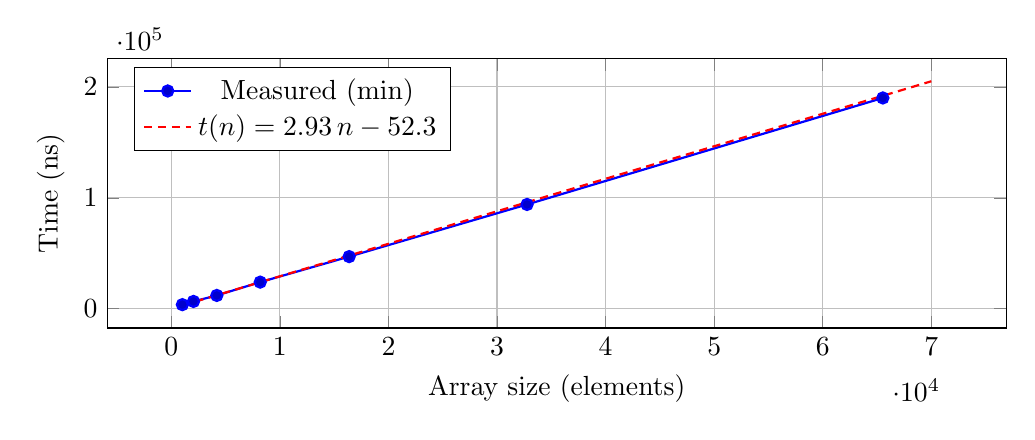
\begin{tikzpicture}
    \begin{axis}[
      xlabel={Array size (elements)},
      ylabel={Time (ns)},
      width=13cm, height=5cm,
      grid=major,
      legend pos=north west,
      ymajorgrids=true,
      xmajorgrids=true
    ]

      % ----------------------------------------------------------
      % Measured MIN times
      % ----------------------------------------------------------
      \addplot+[
        mark=*,
        thick,
        color=blue
      ] coordinates {
        (1024,   3.7e3)
        (2048,   6.6e3)
        (4196,   1.2e4)
        (8192,   2.4e4)
        (16384,  4.7e4)
        (32768,  9.4e4)
        (65535,  1.9e5)
      };
      \addlegendentry{Measured (min)}

      % ----------------------------------------------------------
      % Linear regression fit: t(n) = 2.93 n - 52.3
      % ----------------------------------------------------------
      \addplot[
        red,
        thick,
        densely dashed,
        domain=1000:70000,
        samples=40
      ] {2.93 * x - 52.3};
      \addlegendentry{$t(n)=2.93\,n - 52.3$}

    \end{axis}
  \end{tikzpicture}
  \caption{Minimum measured time per loop with fitted linear regression}
  \label{fig:append-min-times-fitted}
\end{figure}

\subsection*{Benchmark result: Fixed-Variable Append}
Switching the roles of the two linked lists—keeping the first list at a fixed size while allowing the second to grow—results in a constant-time growth pattern, as shown in Figure~2, with the corresponding execution times listed in Table~2. This observation is consistent with the theoretical performance analysis: only the last cell of the fixed linked list must be traversed before the constant-time pointer update can be applied. Consequently, the running time remains bounded by a constant and exhibits an overall time complexity of $O(1)$ for this configuration.

\begin{table}[h]
\begin{center}
\begin{tabular}{l|ccccccc}
\textbf{Size}
    & 1024 & 2048 & 4196 & 8192 & 16384 & 32768 & 65535 \\
\hline
\textbf{Time (ns)}
    & $2.4\times10^{4}$
    & $2.4\times10^{4}$
    & $2.4\times10^{4}$
    & $2.4\times10^{4}$
    & $2.4\times10^{4}$
    & $2.4\times10^{4}$
    & $2.4\times10^{4}$ \\
\end{tabular}
\caption{Minimum time per loop (transposed)}
\label{tab:min-benchmark}
\end{center}
\end{table}

\begin{figure}[h]
  \centering
  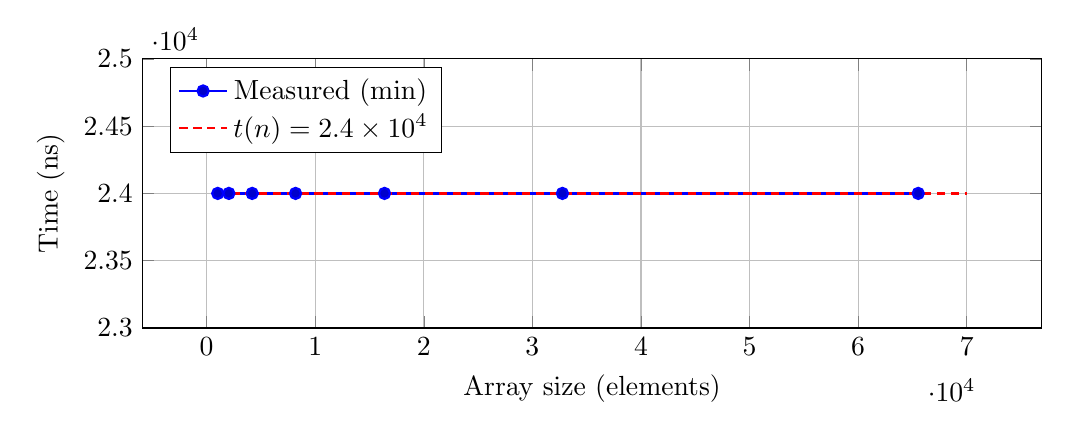
\begin{tikzpicture}
    \begin{axis}[
      xlabel={Array size (elements)},
      ylabel={Time (ns)},
      width=13cm, height=5cm,
      grid=major,
      legend pos=north west,
      ymajorgrids=true,
      xmajorgrids=true,
      ymin=23000,
      ymax=25000
    ]

      % ----------------------------------------------------------
      % Measured MIN times
      % ----------------------------------------------------------
      \addplot+[
        mark=*,
        thick,
        color=blue
      ] coordinates {
        (1024,   2.4e4)
        (2048,   2.4e4)
        (4196,   2.4e4)
        (8192,   2.4e4)
        (16384,  2.4e4)
        (32768,  2.4e4)
        (65535,  2.4e4)
      };
      \addlegendentry{Measured (min)}

      % ----------------------------------------------------------
      % Constant fitted line t(n) = 2.4e4
      % ----------------------------------------------------------
      \addplot[
        red,
        thick,
        densely dashed,
        domain=1000:70000,
        samples=2
      ] {2.4e4};
      \addlegendentry{$t(n)=2.4\times10^{4}$}

    \end{axis}
  \end{tikzpicture}
  \caption{Minimum measured time per loop with fitted constant regression}
  \label{fig:min-times-constant-fit}
\end{figure}

\section*{Comparison with an array}

By comparing performance of a linked list to an array in terms of appending two lists, linked list slightly outperforms arrays. The main reason is that arrays are fixed in size and must be copied into another array when resizing. Appending two arrays requires resizing the first array and copy the elements of the second array into the first one with sufficient space. In this case, the cost of appending two arrays is copying all the elements in both arrays. Assuming the first one has $n$ elements and the second one $m$ elements, the total time complexity is $O(n+m)$. Compared to linked list, the time complexity is only $O(n)$. In Figure~3, linear growth can be visualized with execution time data from Table~3.

\begin{table}[h]
\begin{center}
\begin{tabular}{l|ccccccc}
\textbf{Size}
    & 1024 & 2048 & 4196 & 8192 & 16384 & 32768 & 65535 \\
\hline
\textbf{Time (ns)}
    & $2.0\times10^{4}$
    & $2.2\times10^{4}$
    & $2.7\times10^{4}$
    & $4.5\times10^{4}$
    & $6.2\times10^{4}$
    & $8.3\times10^{4}$
    & $1.5\times10^{5}$ \\
\end{tabular}
\caption{Minimum time per loop vs. input size (transposed)}
\label{tab:min-times-latest}
\end{center}
\end{table}

\begin{figure}[h]
  \centering
  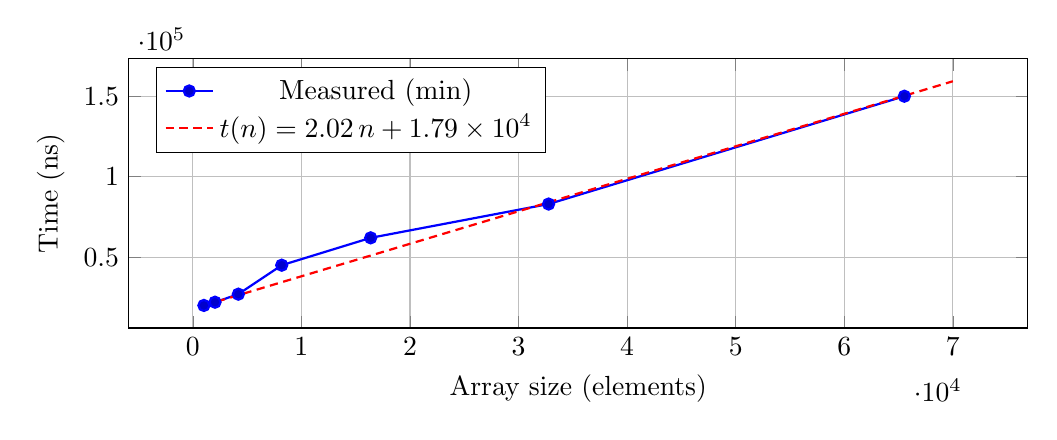
\begin{tikzpicture}
    \begin{axis}[
      xlabel={Array size (elements)},
      ylabel={Time (ns)},
      width=13cm, height=5cm,
      grid=major,
      legend pos=north west,
      ymajorgrids=true,
      xmajorgrids=true
    ]

      % ---------------------------
      % Measured MIN times
      % ---------------------------
      \addplot+[
        mark=*,
        thick,
        color=blue
      ] coordinates {
        (1024,   2.0e4)
        (2048,   2.2e4)
        (4196,   2.7e4)
        (8192,   4.5e4)
        (16384,  6.2e4)
        (32768,  8.3e4)
        (65535,  1.5e5)
      };
      \addlegendentry{Measured (min)}

      % ---------------------------
      % Linear fit: t(n) ≈ 2.02 n + 1.79e4
      % Keep domain small to avoid timeouts
      % ---------------------------
      \addplot[
        red,
        thick,
        densely dashed,
        domain=1000:70000,
        samples=40
      ] {2.02 * x + 1.79e4};
      \addlegendentry{$t(n)=2.02\,n + 1.79\times10^{4}$}

    \end{axis}
  \end{tikzpicture}
  \caption{Minimum time per loop with fitted linear trend}
  \label{fig:min-times-latest}
\end{figure}

\section*{Stack implementation using linked list}

A stack can also be implemented using a linked list. The elements are pushed to the first position in the linked list, which can thereafter be popped by removing the first element of the list and returning its value. The push operation is implemented exactly the same as adding an element into the first position of the linked list. However, the pop operation requires first removing the first element from the linked list stack, by updating the pointer to first element cell to point to the second element, while de-allocating the first element.

\begin{minted}{c}
void linked_stack_push(linked_stack *lnk, int item) {
    // same as inserting element into first position in linked list
}

int linked_stack_pop(linked_stack *lnk) {
    if (lnk->first == NULL) {
        return 0;
    }
    // Remove first element
    linked_stack_cell *first_cell = lnk->first;
    int value = first_cell->value;
    lnk->first = lnk->first->tail;
    free(first_cell);
    return value;
}
\end{minted}

Although a linked‑list stack grows flexibly without resizing, it is slower in practice. Both array‑based and linked‑list stacks have amortized $O(1)$ push/pop time, but linked lists suffer from pointer chasing, cache misses, and allocation overhead. Arrays use contiguous memory with cheap reads and writes, so they generally outperform linked lists despite identical asymptotic complexity.

\section*{Conclusion}

Linked lists in C provide structural flexibility with inexpensive insertions and deletions, while arrays benefit from contiguous memory layouts and superior cache performance. Searching in a linked list requires linear time $O(n)$, whereas insertion or deletion is $O(1)$ when the pointer to the target cell is already known.

In the first benchmark, the size of linked list $a$ was varied while it was appended to a fixed-size list $b$. Without a tail pointer, the append operation must traverse all $n$ elements of $a$, giving a linear running time of $O(n)$, which matches the measured results.

In the second benchmark, the size of $a$ was fixed while the size of $b$ increased. Because the append operation only traverses the fixed list before a constant-time pointer update, the running time remains constant, showing an overall complexity of $O(1)$.

For arrays, appending requires allocating a new array of size $n+m$ and copying all elements, resulting in a time complexity of $O(n + m)$. Linked lists avoid this full copy and only require traversal of the destination list; with a tail pointer, even this becomes $O(1)$.

\begin{table}[h]
\centering
\begin{tabular}{l|p{5cm}|p{5cm}}
\textbf{Aspect} 
    & \textbf{Linked list} 
    & \textbf{Array} \\ \hline

Variable-fixed append 
    & Traverses $n$ nodes; $O(n)$ 
    & Copy $n+m$ elements; $O(n+m)$ \\ \hline

Fixed-variable append
    & Traverses fixed list; $O(1)$ 
    & Still copies $n+m$ elements; $O(n+m)$ \\ \hline

Memory behavior
    & Non-contiguous; weaker locality 
    & Contiguous; strong locality \\ \hline

Practical performance
    & Flexible but slower  
    & Typically faster \\ \hline
\end{tabular}
\caption{Benchmark-based comparison of linked lists and arrays}
\label{tab:ll-vs-array}
\end{table}

Overall, linked lists trade memory locality for structural flexibility, while arrays achieve faster practical performance through contiguous storage and efficient memory access patterns.

\end{document}